\documentclass[12pt, a4paper]{article}
\pagenumbering{arabic}
\usepackage[utf8]{inputenc}
\usepackage[T1]{fontenc}
\usepackage{geometry}
\usepackage{graphicx}
\graphicspath{{images/}}
\geometry{a4paper}
\usepackage{helvet}
\newcommand\tab[1][1cm]{\hspace*{#1}}
\renewcommand{\familydefault}{\sfdefault}
\setlength{\topmargin}{-2cm}
\setlength{\oddsidemargin}{0cm}
\setlength{\textheight}{24cm}
\setlength{\textwidth}{16cm}
\usepackage{graphicx}
\usepackage{listings}
\usepackage{sectsty}
%Use Helvetica as the sansserif font
\usepackage{helvet}
%Use sffamily for all titles
\allsectionsfont{\sffamily}

\begin{document}
\begin{titlepage}
    \vspace*{\fill}
    \begin{center}
      \Huge{\textbf{HOSTELS}}\\[2cm]
      \Large{Opio Emmanuel Omona}\\[1cm]
      $20^{th} May, 2017$\\[1cm]
      \normalsize {Report On The Various Hostels Around Makerere University}
    \end{center}
    \vspace*{\fill}
\end{titlepage}

\Large{\textbf{Acknowledgements}}\\
\small
We would like to thank the following people for their contribution to the research and preparation of this report:
\begin{enumerate}
\item All those who contributed through interviews.
\item Classmates that helped in configuring the online server\\
\end{enumerate}

\Large{\textbf{Abstract}}\\
\small
This research was conducted about hostels around Makerere University for the purpose of gathering information about the attributes of various Hostels so as to guide students on what to look for when picking a hostel. Often students join campus as freshers and pick hostels without knowing what the merits and demerits of that hostel are. Residents of the hostels provided some of the information about their respective hostels and that allowed me complete my research succesfully.

\tableofcontents
\clearpage
\renewcommand{\theenumi}{\pagenumbering{roman}}
\section{INTRODUCTION AND PROBLEM STATEMENT}

\subsection{Background of the study}
The research was conducted partly because of past problems or experiences that the author faced. As a freshman, the author moved from Hostel to Hostel looking for his preferences. Therefore the author decided to make research about the topic named above so as to prevent other freshmen from falling victim of circumstance.

\subsection{Statement of the problem}
Often when one joins campus, one is unaware and ignorant about many things including knowledge about hostels, to mention but a few. This research is meant to answer the question most freshmen ask to the themselves; Which hostel should i go to? This is based on a few parameters like the cost, distance from the campus, security among many others.

\subsection{Objectives}
As alluded to in the problem statement, the key objective of this study is to find out the best Hostel that suits an individual.\\
To achieve this objective a study was needed which aimed to collect information necessary to scale a difference among all the Hostels around Makerere University.\\
Due to time and cost constraints however it was not possible to gather all the necessary informtion about all the hostels to achieve this objective.  It was therefore necessary to identify a sample of Hostels that could be used to achieve this goal.

\subsection{Scope}
Geographically, the research was intended to cover all the regions around Makerere, that includes Kikoni, Kikumi kikumi, Katanga and Wandegeya. Unfortunately due to some limitations that are expressed in the limitations section, the geographical scope was reduced to Kikoni, Katanga and Kikumi Kikumi.

\subsection{Delineations And Limitations}
In a study of this nature it is important to clearly delineate the objectives of the study.  The most important delineation is in the limitation of scope, which has been expressed in the objectives.\\  
Some of the limitations in this research include:\\
The fact that the research was not funded and purely on the expense of the researcher. Some of the expenses include buying data(internet) bundles, external storage devices to store the data collected, transport, among other costs.\\
Since some of the data collected required GPS coordinates, the internet connection wasn't so good which led rise to incorrect results.\\
In addition certain tools were hard to configure and this took a big portion of the time to do this reserach.

\clearpage

\section{LITERATURE REVIEW}
The purpose of this research was to provide information to the users about the various Hostels. However, a similar research has been conducted according to [1] where some of the information in this resaerch was got. The cited artcle covered information about the prices of some of the hostels. Prices of hostels that were not in that article were got from some of the residents through interviews.\\
This research also builds on the former by including the GPS locations of Hostels that is latitude and longitude as well as the degree of accuracy. In addition the research also includes various other data.

\section{METHODOLOGY}
\subsection{Introduction}
The purpose of this chapter is to give an account of the approach followed to test and conclude on the research problems presented in this study. The chapter begins by discussing the choice of research design for the study. Next the research methodology, which details how the questionnaire for this study was developed, which data sources were used, how the sample was selected and how the data was collected, coded and analysed, is described.

\subsection{Research Design}
The choice of research design is generally influenced by the research objectives and the nature of the research problems to be solved.  In situations where the research problem has been the subject of earlier studies, cognisance would for example be given to how that research problem had previously been researched.\\
The research used both qualitative and qualitative methods to answer the research questions. The following table summarises the methods used to answer each question:

\begin{center}
\begin{tabular}{||c | c||}
\hline \textbf{Research Question} & \textbf{Method Used To Answer Question}\\
[0.5ex]
\hline
\hline Name of Hostel & Observation\\
\hline Location & GPS\\
\hline How far from Campus & Measurements\\
\hline How would you rate this Hostel & Interview\\
\hline What is the price of the rooms & Interview\\
\hline Is there a shuttle & Interview\\
[0.5ex]
\hline 
\end{tabular}
\end{center}

\subsection{Instuments}
Observations were got by taking pictures using a camera. The Interviews were conducted in person, however they were not recorded. Questionnaires were got from a form which is shown in the picture below. The GPS Location was got using google maps through an application on an Android Platform. The Measurements were also got using a distance measurement application which is also shown in the picture below. Most of these methods used a mobile application called ODK collect (Open Data Kit).
\clearpage
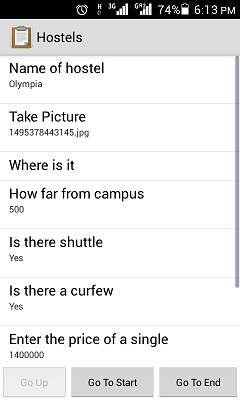
\includegraphics{capture}

\subsection{Sample}
The sample of Hostels was selected by distribution, that is atleast one Hostel from each geographical location was selected to carry out this research. In addition there was some level of finance that influenced the hostels to be picked i.e hostels of all economic classes were chosen to be picked.

\subsection{Data Collection}
The Data was collected by the author of this report. It was collected face-to-face and in English which was the first language of many of the participants. The data was collected on at a time, moving through the different regions.

\clearpage
\section{Results And Analysis}
The results of the research are shown and explained in the graphs below.

\subsection{How Far From Campus}
The graph below shows the relative distances of all the campuses from the the campus. This information can help you know how much time it can take you to reach the campus. However some information like the whether or not the hostel has a shuttle was collected and was stored in an a server online[2]. As you can see Nana Hostel is the furthest as compared to Kasamba Hostel.\\
\\
\includegraphics{Chart}

\subsection{How Much Is A Room}
The Graph below shows the Average Prices of some of the hostels as it was taken during the middle of the research. The longest graph shows the most price. 1 stands for Olympia, 2 - Nana, 3 - Hollywood, 4 - Kasamba and 5- MISH.\\
The prices can help the reader determine which Hostel to choose based on the readers' economic status.\\
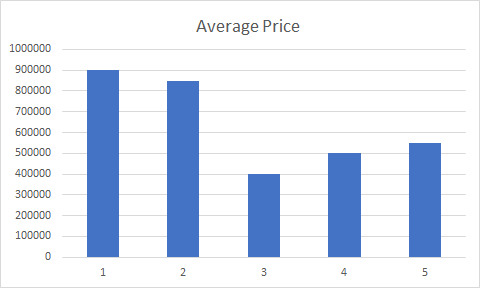
\includegraphics{Graph}

\section{Conclusion}
This research was succesfully completed, and the report was written. The research was to determine which Hostel would be most suitable. A definite order couldn't be determined as there are many parameters that are  based on preference per user. Therefore each reader is do deteremine which Hostel best suits them.

\newpage
\section{References}
$[1] http://campuseye.ug/top-10-hostels-in-makerere-kikoni$\\
$[2] http://www.research-167909.appspot.com $\\
\end{document}